\paragraph{\bf Réponse.} \\

On raisonne par \emph{données virtuelles} : 
\begin{itemize}
\item L'{\it a priori} non-informatif de Jeffreys est utilisé pour modéliser l'absence d'expertise et la simple connaissance du modèle 
\begin{eqnarray*}
\pi_{0}(\lambda) & \propto \lambda^{-1}  \ \ \ \ \ \ \ \ \text{ {\it (paramètre d'échelle)}}. 
\end{eqnarray*} 
\item L'information apportée par l'expert est assimilée à celle apportée par un échantillon i.i.d. 
\begin{eqnarray*}
{\bf x_m} & \sim & {\cal{E}}(\lambda).
\end{eqnarray*}
\item Un ``bon" prior informatif pour $\lambda$ est donc $\pi(\lambda)=\pi_0(\lambda|{\bf x_m})$, soit
\begin{eqnarray*}
\lambda & \sim & {\cal{G}}(m,m \bar{\bf x}_m).
\end{eqnarray*} 
\end{itemize}
Donc $2m \bar{\bf x}_m \lambda \sim {\cal{G}}(m,1/2) \equiv \chi^2_{2m}$, d'où ${\displaystyle \bar{\bf x}_m  =  \frac{\chi^2_{2m}(\alpha)}{2m\bar{\lambda}}}$. Le décideur peut fixer arbitraitement $m$ selon la confiance qu'il a en l'expert {(ou mettre un {\it a priori} hiérarchique dessus)}. De plus, l'{\it a priori} est \emph{conjugué} : sachant des durées de vie observées ${\bf x_n}=(x_1,\ldots,x_n)$, la loi {\it a posteriori} de $\lambda$ est
\begin{eqnarray*}
\lambda|{\bf x_n} & \sim & {\cal{G}}\left(m+n,\frac{\chi^2_{2m}(\alpha)}{2\bar{\lambda}} + n\sum\limits_{i=1}^n x_i\right)
\end{eqnarray*} 
L'ingénieur s'intéresse alors à la probabilité \emph{prédictive} que $\Sigma$ tombe en panne avant la prochaine visite au temps $x_0$
\begin{eqnarray*}
P\left(X<x_0\right)  & = & \int_{0}^{\infty} P\left(X<x_0|\lambda\right) \pi(\lambda|{\bf x_n}) \ d\lambda \ = \ 
                   1 - 1/\left(1 + \frac{x_0}{\frac{\chi^2_{2m}(\alpha)}{2\bar{\lambda}} + n\sum\limits_{i=1}^n x_i}\right)^{m+n}
\end{eqnarray*}
puis il peut introduire une fonction de co\^ut, etc. pour prendre une décision. Les figures suivantes (\ref{expert1} à \ref{expert3}) illustrent ainsi différents comportements {\it a posteriori}, lorsqu'on simule 10 données selon ${\cal{E}}(\lambda_0)$ avec $\lambda_0=1/10$. \\ 

\begin{figure}[h!]
\centering
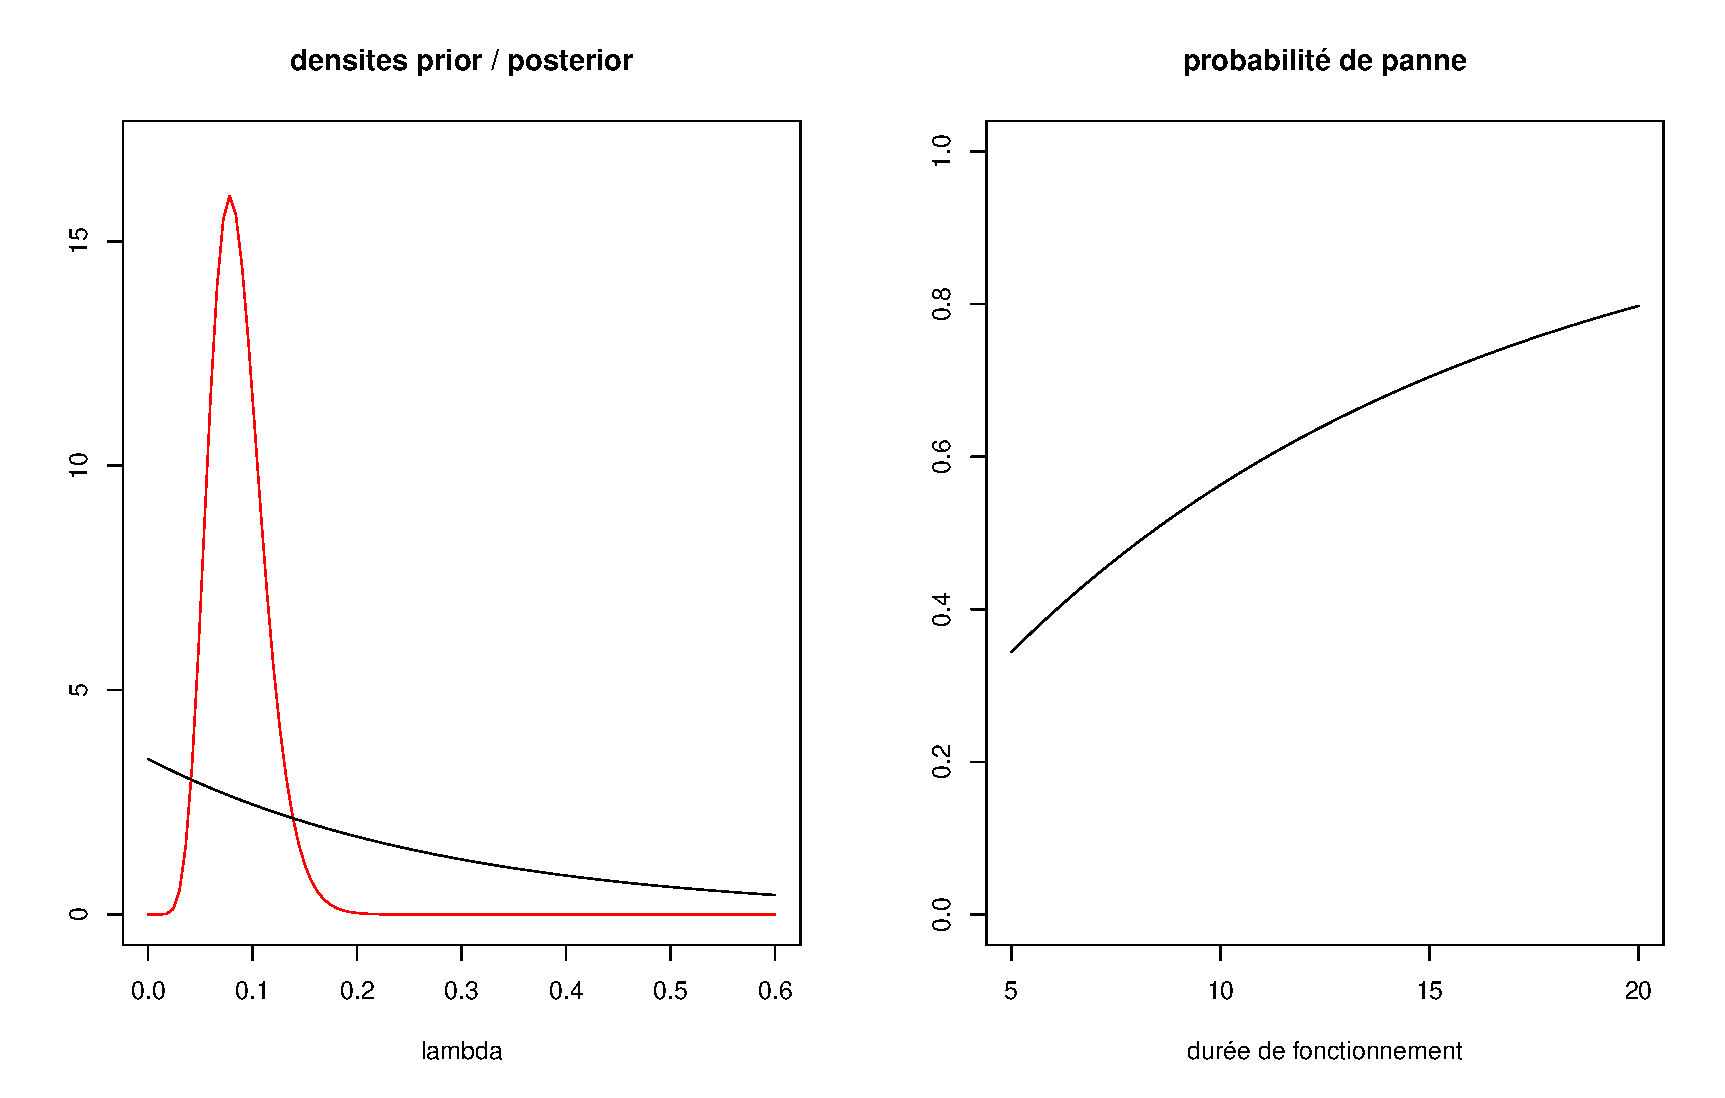
\includegraphics[scale=0.4]{figures/prior/figure01.pdf} 
\caption{$m=1$, $\bar{\lambda}=1/5$, $\alpha=50\%$ (expert peu informatif et pessimiste).}
\label{expert1}
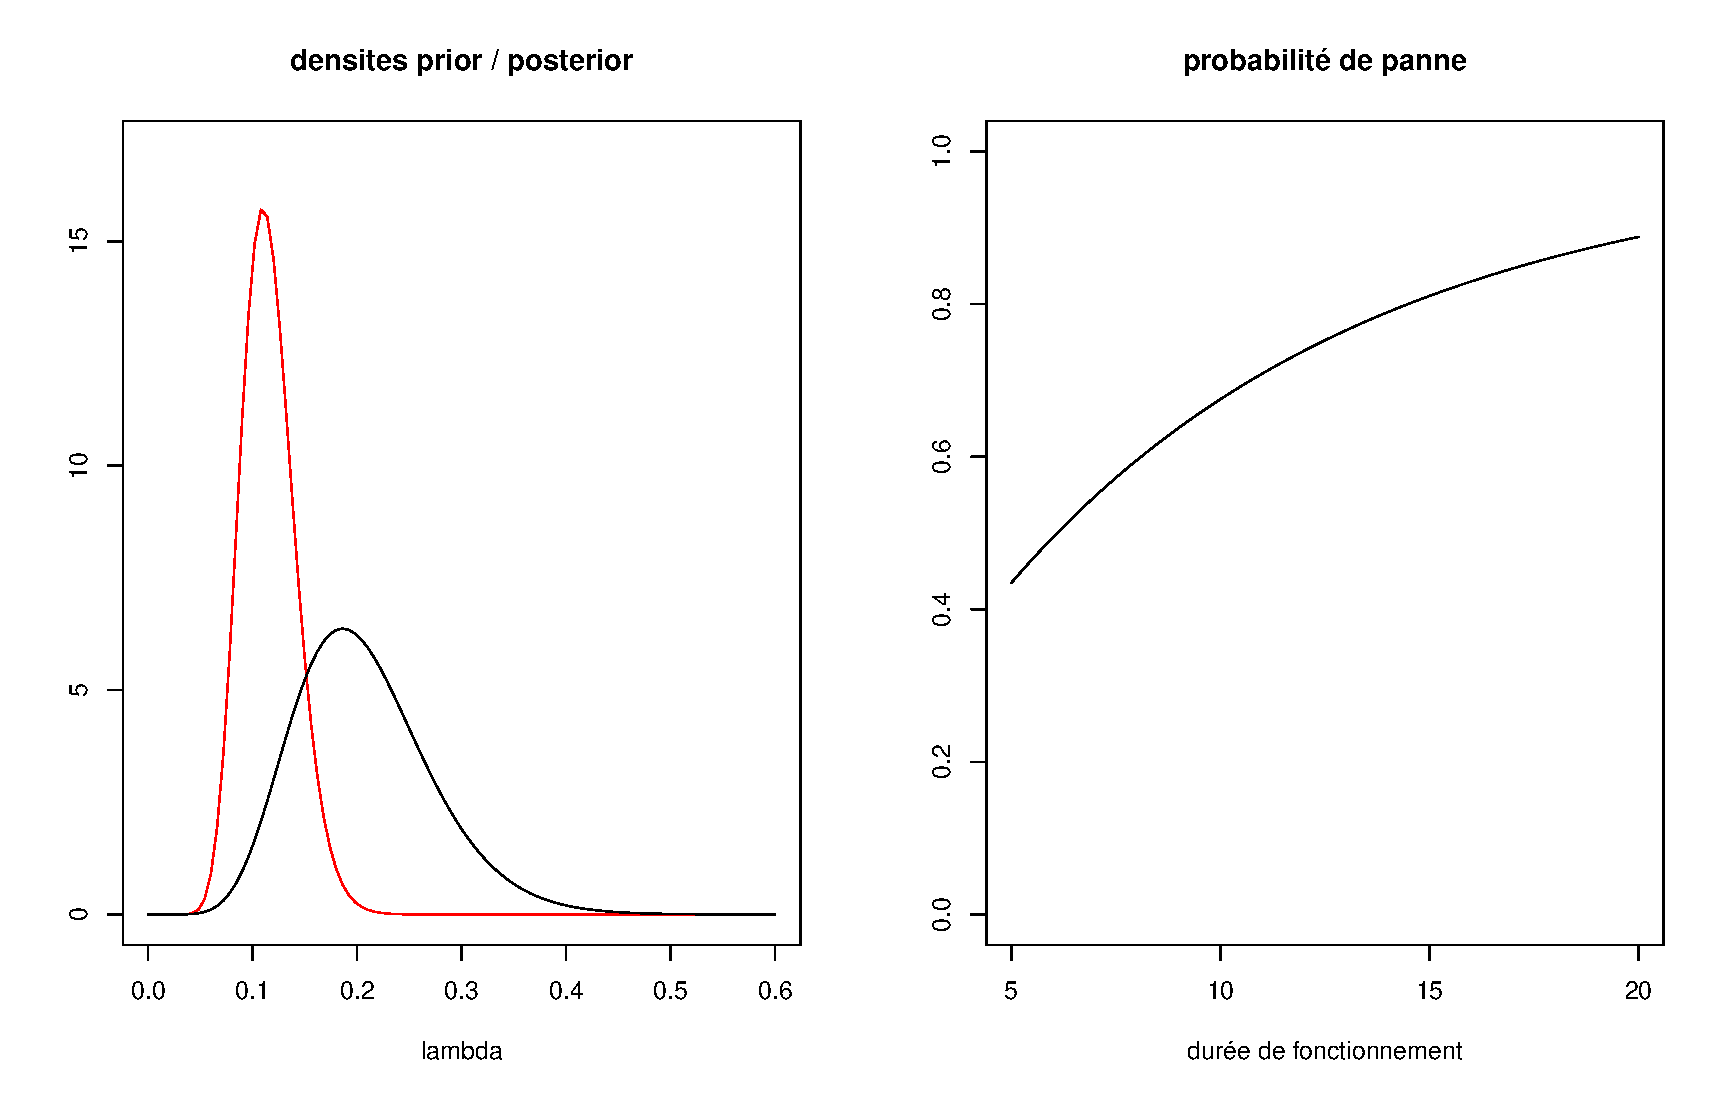
\includegraphics[scale=0.4]{figures/prior/figure02.pdf} 
\caption{$m=10$, $\bar{\lambda}=1/5$, $\alpha=50\%$ (expert très informatif et pessimiste).} \label{expert2}
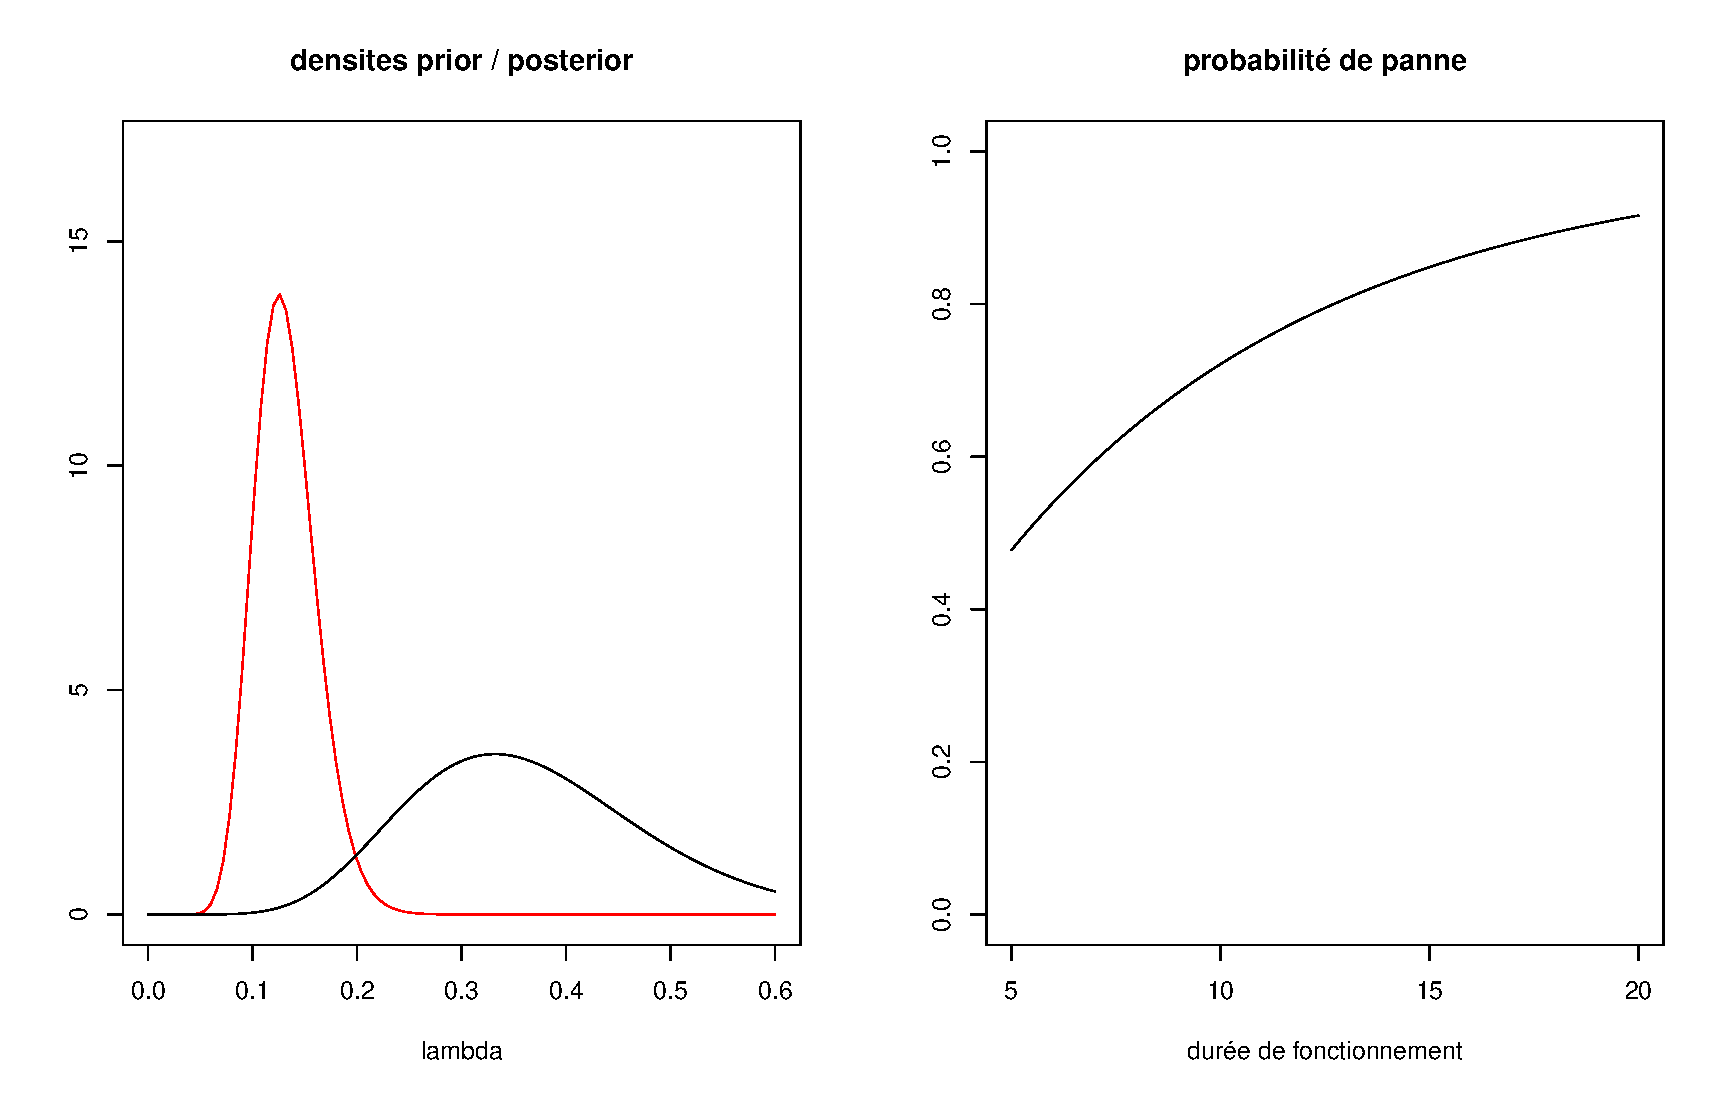
\includegraphics[scale=0.4]{figures/prior/figure03.pdf} 
\caption{$m=10$, $\bar{\lambda}=1/5$, $\alpha=5\%$ (expert très informatif et très pessimiste).} \label{expert3}
\end{figure}

En fait, plus habituellement, l'expert préfère exprimer son opinion \emph{quantitative} sur la durée de vie $X$
 ($=$ \emph{variable d'ancrage}) que sur $\lambda$, car $X$ est {\bf observable}. Dans ce cas, il est assimilé à un fournisseur d'estimé du \emph{quantile prédictif {\it a priori}} $\bar{x}$ :
\begin{eqnarray*}
\int_{0}^{\bar{x}} f(x) \ dx & = & \int_{0}^{\bar{x}} \int_{\Theta} f(x|\theta)\pi(\theta) \ d\theta \ = \ \alpha
\end{eqnarray*}
Cette interprétation est la plus acceptée en général dans la communauté statistique bayésienne, c'est pourquoi les statisticiens fiabilistes préfèrent poser des questions comme : 
\begin{eqnarray*}
\text{\it Sachant les temps $x_0$ et $x_1>x_0$, $\Sigma$ a $1-\alpha$ fois plus de chance de ne pas tomber en panne après $x_0$ qu'après $x_1$.} \\
\text{\it Quelle est votre évaluation de $1-\alpha$ ?} 
\end{eqnarray*}
%\item La réponse est un estimé de $\P(X>x_0)/P(X>x_1)$
